
\chapter{Brownian Motion}


\section{Historical observations}
The history of Brownian motion dates back to the early observations of the botanist Robert Brown. While observing pollen grains suspended in a liquid, he noted their highly erratic and jagged trajectory. These particles were subsequently named \textit{Brownian} particles.


\begin{figure}[h!]
    \centering
    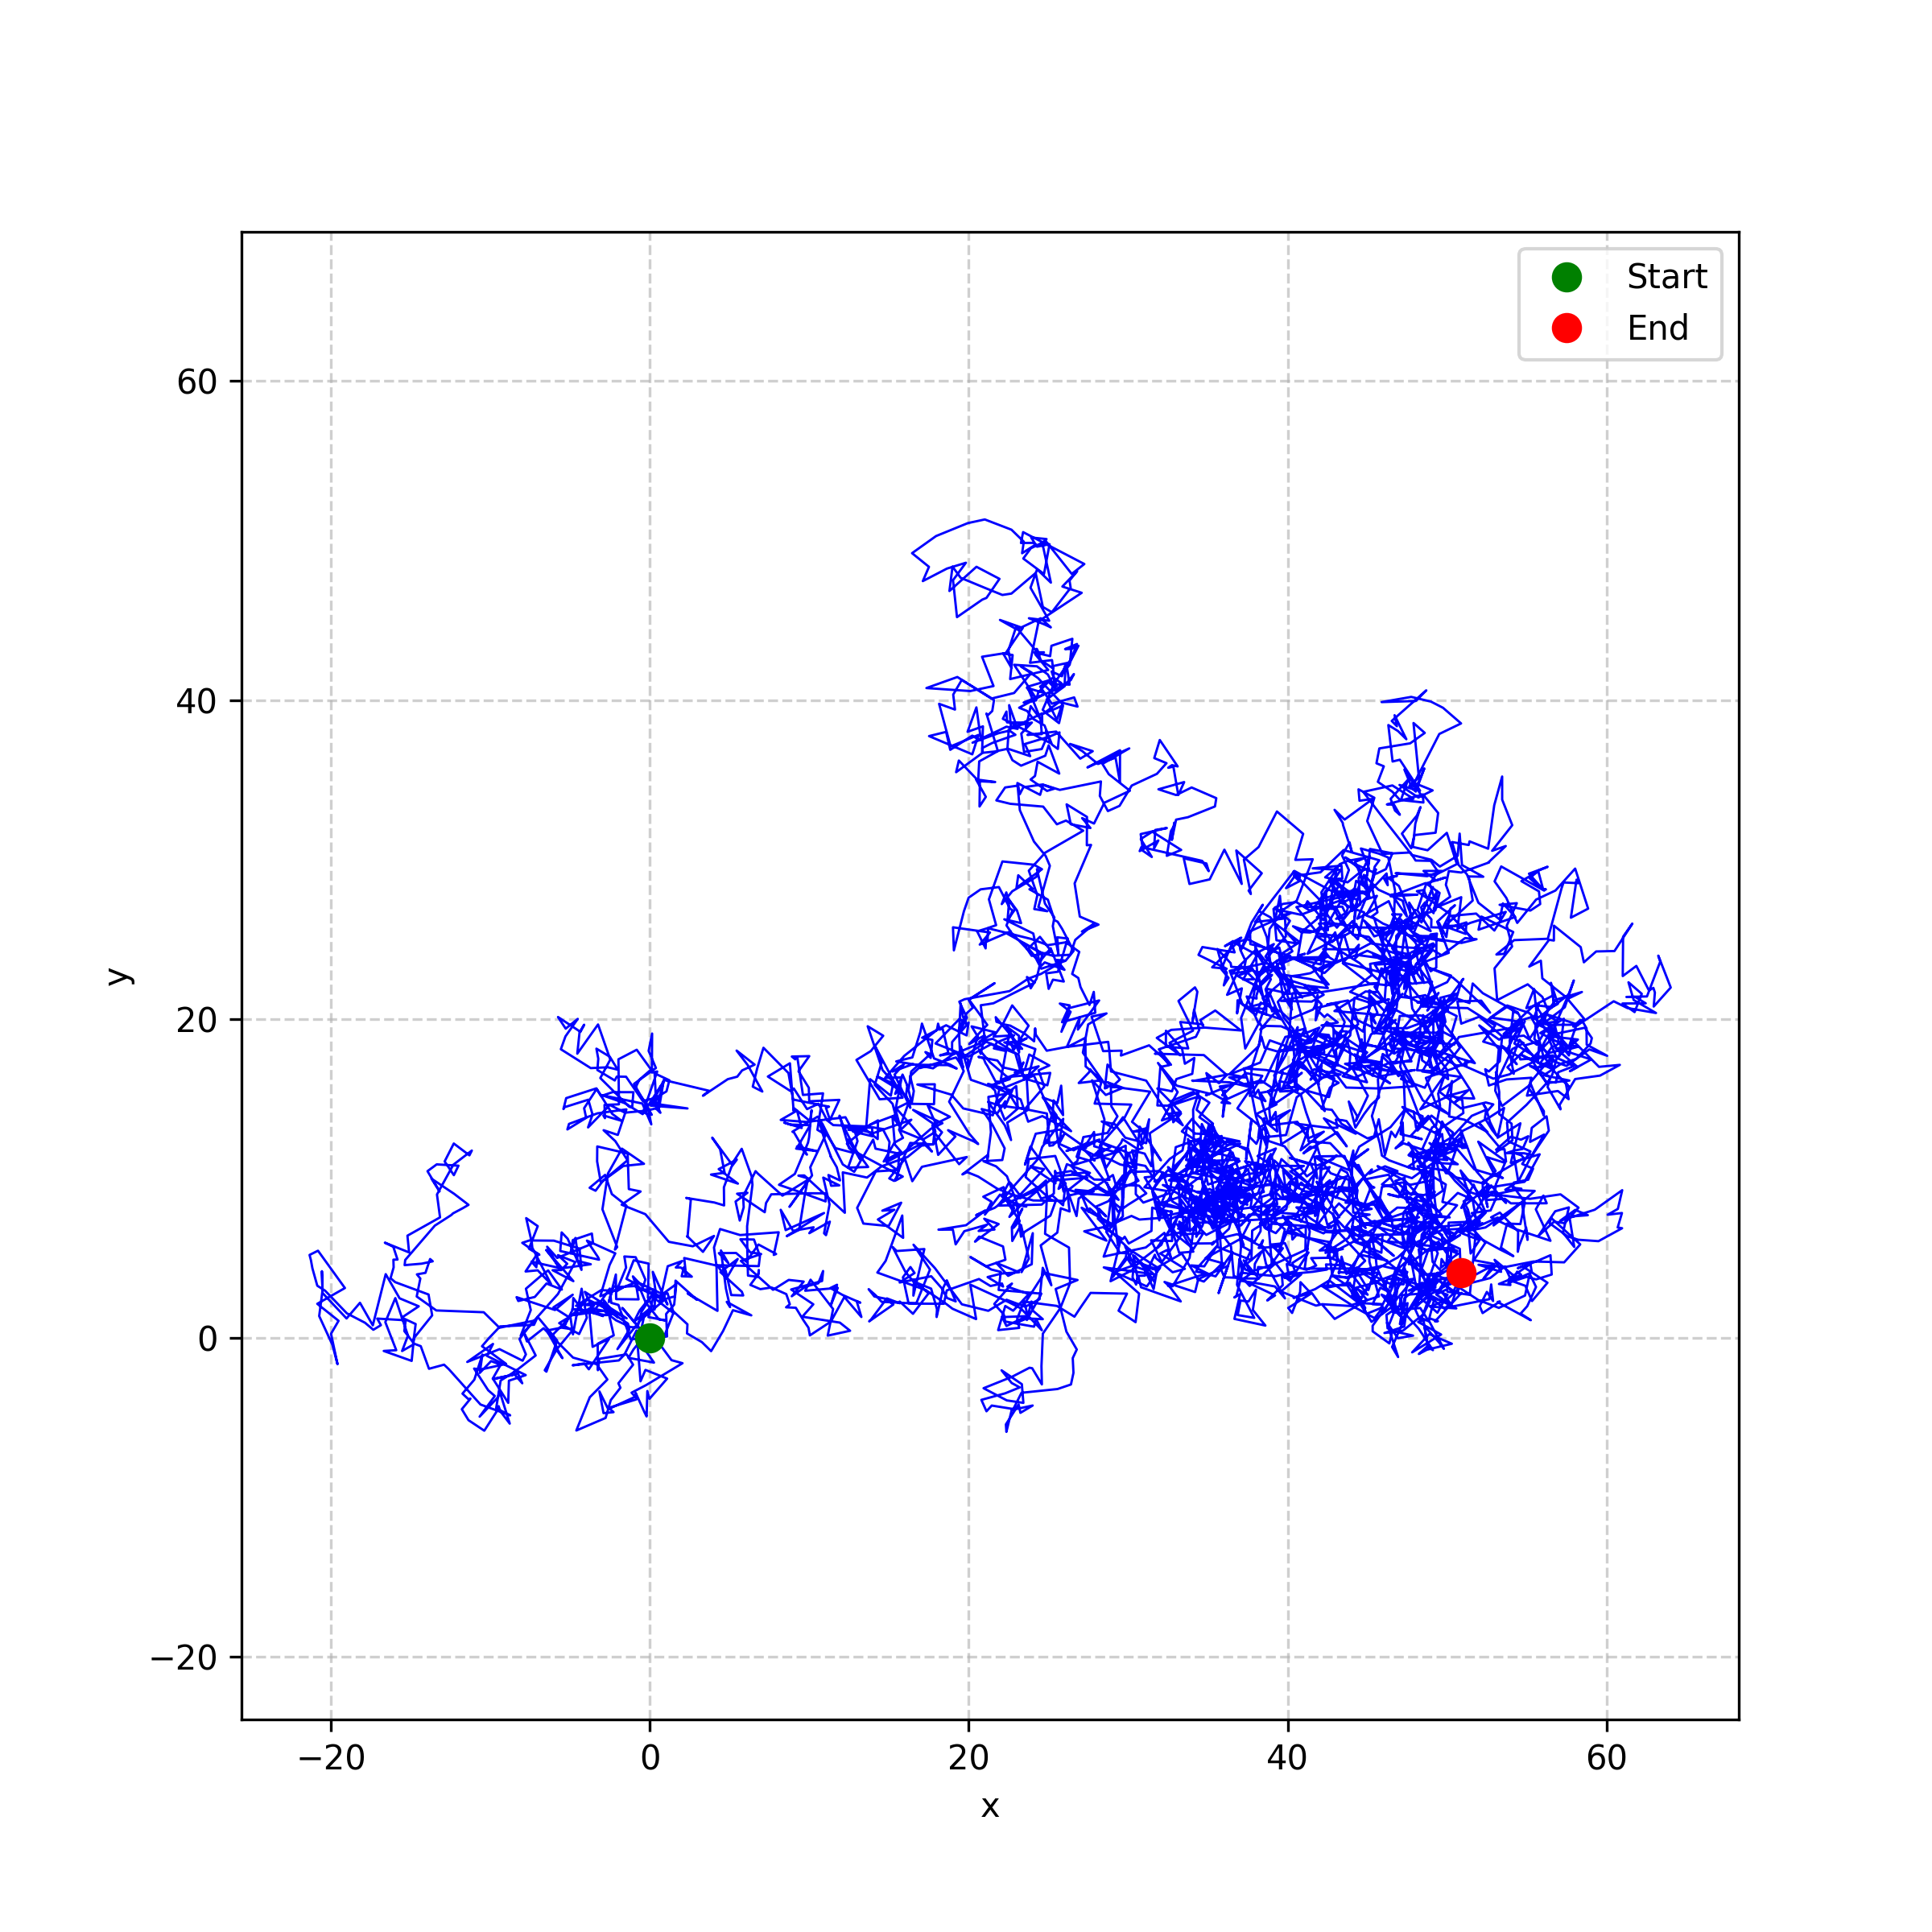
\includegraphics[width=0.6\textwidth]{images/brownian_motion_2d.png}
    \caption{Simulation of a Brownian trajectory in two dimensions.}
\end{figure}

Specifically, Brown made the following qualitative observations:
\begin{enumerate}[label=\roman*)]
    \item The motion never seems to cease.
    \item Different particles always move independently of one another.
    \item The particle's material composition (organic or inorganic) or its mass density do not seem to matter.
    \item The motion becomes faster and more agitated as the fluid's temperature increases or as its viscosity decreases.
    \item The motion exhibits scale invariance (it looks similarly jagged at different magnifications).
    \item The trajectory appears to have no tangent at any point.
\end{enumerate}

The first theoretical characterization of this phenomenon was provided by Albert Einstein in two revolutionary papers published in 1905 \cite{Einstein1905, Einstein1906}. We will now illustrate the key steps of his reasoning.
\section{Einstein's papers}
\subsection{From random walk to the diffusion equation}
He considered a one-dimensional, infinitely extended fluid composed of an ensemble of particles. The Brownian particle undergoes a series of discrete displacements, or "jumps", over very small, successive time intervals, denoted by $\tau$, much smaller than the observation time $T$.


\begin{center}
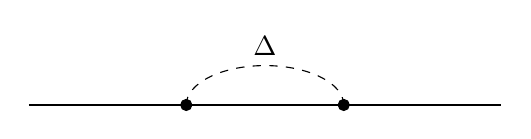
\begin{tikzpicture}

  \draw[thick] (-3,0) -- (3,0);

  \filldraw[black] (-1,0) circle (2pt);
  \filldraw[black] (1,0) circle (2pt);

  \draw[dashed] (-1,0) arc (180:0:1cm and 0.5cm);

  \node[above] at (0,0.5) {$\Delta$};
\end{tikzpicture}
\end{center}

To describe the statistics of these jumps, Einstein introduced an auxiliary function, $\phi(\Delta)$, which is the probability density function (PDF) for a jump of magnitude $\Delta$. The term $\phi(\Delta)d\Delta$ represents the probability that a single jump has a magnitude between $\Delta$ and $\Delta+d\Delta$. This function is defined by two fundamental properties based on physical reasoning:
\begin{itemize}
    \item \textbf{Normalization}: The particle must perform a jump of some magnitude, so the total probability over all possible jumps must be equal to 1. This is expressed by the normalization condition:
    \begin{equation}
    \int_{-\infty}^{\infty} \phi(\Delta) \,d\Delta = 1.
    \end{equation}
    \item \textbf{Symmetry}: In the absence of any external force or drift, the fluid is isotropic. Therefore, a jump to the right ($+\Delta$) is as probable as a jump of the same magnitude to the left ($-\Delta$). This implies that the function $\phi$ must be an even function:
    \begin{equation}
    \phi(\Delta) = \phi(-\Delta).
    \end{equation}
\end{itemize}

The main goal, however, is to find $p(x,t)$, which represents the number of particles per unit length at position $x$ and time $t$. If we consider $p(x,t)$ as the probability density for a single particle, it must be normalized such that its integral over all space is 1:
\begin{equation}
\int_{-\infty}^{\infty} p(x,t) \,dx = 1.
\end{equation}
The probability of finding the particle in the infinitesimal interval $[x, x+dx]$ is therefore $p(x,t)dx$.

The core idea is to relate the particle density at time $t_f = t+\tau$ to the density at time $t_i = t$. The density of particles at position $x$ at the future time $t+\tau$, denoted $p(x, t+\tau)$, is the sum of probabilities of particles arriving at $x$ from all possible previous positions. A particle that ends up at $x$ must have been at a position $x+\Delta$ at time $t$ and then performed a jump of size $\Delta$. Summing over all possible jumps $\Delta$:
\begin{equation}\label{eq:einstein-master}
p(x, t+\tau) = \int_{-\infty}^{\infty} P(x+\Delta, t) \phi(\Delta) \,d\Delta.
\end{equation}

Now, we perform a Taylor expansion for small $\tau$ and small $\Delta$. The left side is expanded in time:
\begin{equation}
p(x, t+\tau) \approx p(x,t) + \tau \frac{\partial p(x,t)}{\partial t} + \dots;
\end{equation}
the term $p(x+\Delta, t)$ inside the integral is expanded in space around the position $x$:
\begin{equation}
p(x+\Delta, t) \approx p(x,t) + \Delta \frac{\partial p(x,t)}{\partial x} + \frac{\Delta^2}{2} \frac{\partial^2 p(x,t)}{\partial x^2} + \dots;
\end{equation}
substituting these expansions back into Equation~\eqref{eq:einstein-master}:
\begin{equation}
p(x,t) + \tau \frac{\partial P}{\partial t} \approx \int_{-\infty}^{\infty} \left[ p(x,t) + \Delta \frac{\partial p}{\partial x} + \frac{\Delta^2}{2} \frac{\partial^2 p}{\partial x^2} \right] \phi(\Delta) \,d\Delta.
\end{equation}
We can split the integral by linearity:
\begin{equation}
p(x,t) + \tau \frac{\partial p}{\partial t} \approx p(x,t) \underbrace{\int \phi(\Delta)d\Delta}_{=1} + \frac{\partial p}{\partial x} \underbrace{\int \Delta \phi(\Delta)d\Delta}_{=0} + \frac{1}{2}\frac{\partial^2 p}{\partial x^2} \int \Delta^2 \phi(\Delta)d\Delta.
\end{equation}
The terms simplify based on the properties of $\phi$.

So we are left with:
\begin{equation}
\tau \frac{\partial p(x,t)}{\partial t} \approx \frac{1}{2}\frac{\partial^2 p(x,t)}{\partial x^2} \int_{-\infty}^{\infty} \Delta^2 \phi(\Delta) \,d\Delta.
\end{equation}
Dividing by $\tau$, we get:
\begin{equation}
\frac{\partial p(x,t)}{\partial t} = D \frac{\partial^2 p(x,t)}{\partial x^2}.
\end{equation}
This is the \emph{diffusion equation} (with $D=1$ it becomes the well known heat equation), where $D$ is the \emph{diffusion coefficient}, defined as:
\begin{equation}
D := \frac{1}{2\tau} \int_{-\infty}^{\infty} \Delta^2 \phi(\Delta) \,d\Delta.
\end{equation}
Since $\Delta^2 \ge 0$ and $\phi(\Delta) \ge 0$, the integral is positive, thus $D>0$. The dimensions of $D$ are length squared per unit time, $[D] = L^2 T^{-1}$.


\subsection{Solution of the diffusion equation}
We now solve the diffusion equation with a specific initial condition. Physically, it is natural to assume that the process starts with the particle (or all particles) located exactly at the origin at time $t=0$. This condition is represented mathematically by the Dirac delta function, $\delta(x)$. It represents an instantaneous, infinitely concentrated point source. The solution $p(x,t)$ will then describe how this initial certainty "diffuses" into a probability distribution over time.

The problem is thus defined by the partial differential equation and its initial condition:
\begin{equation}\begin{split}
    \frac{\partial p(x,t)}{\partial t} &= D \frac{\partial^2 p(x,t)}{\partial x^2}; \\
    p(x,0) &= \delta(x).
\end{split}\end{equation}
We solve this using the Fourier transform. Let $p(k,t)$ be the Fourier transform of $p(x,t)$ with respect to the spatial variable $x$. The transform pair is defined as:
\begin{equation}\begin{split}
    \text{Inverse Transform:} \quad p(x,t) &= \int_{-\infty}^{\infty} e^{ikx} p(k,t) \,dk; \\
    \text{Transform:} \quad p(k,t) &= \frac{1}{2\pi} \int_{-\infty}^{\infty} e^{-ikx} p(x,t) \,dx.
\end{split}\end{equation}
First, we transform the initial condition. Using the integral representation of the Dirac delta, $\delta(x) = \frac{1}{2\pi} \int e^{ikx} dk$,
\begin{equation}
p(k,0) = \frac{1}{2\pi}.
\end{equation}
Next, we transform the diffusion equation itself. The time derivative remains, while the spatial derivative becomes a multiplication by $(ik)^2 = -k^2$:
\begin{equation}
\mathcal{F}\left[\frac{\partial p}{\partial t}\right] = D \cdot \mathcal{F}\left[\frac{\partial^2 p}{\partial x^2}\right] \implies \frac{\partial p(k,t)}{\partial t} = D(-k^2)p(k,t).
\end{equation}
This transforms the partial differential equation in $(x,t)$ into a simpler ordinary differential equation in the variable $t$ for each value of $k$:
\begin{equation}\begin{split}
    \frac{\partial p(k,t)}{\partial t} &= -Dk^2 p(k,t); \\
    p(k,0) &= \frac{1}{2\pi}.
\end{split}\end{equation}
This is a first-order linear ODE with constant coefficients, which can be solved by separation of variables.

Let's treat $k$ as a constant parameter and solve the ODE for the function $f(t) = p(k,t)$:
\begin{equation}
\frac{df(t)}{dt} = (-Dk^2) f(t).
\end{equation}
Separating the variables $f$ and $t$:
\begin{equation}
\frac{df}{f} = -Dk^2 \,dt.
\end{equation}
Integrating both sides:
\begin{equation}
\int \frac{1}{f} \,df = \int -Dk^2 \,dt \implies \ln|f| = -Dk^2 t + C_0.
\end{equation}
where $C_0$ is the constant of integration. Exponentiating both sides gives:
\begin{equation}
f(t) = e^{-Dk^2 t + C_0} = e^{C_0} e^{-Dk^2 t} = C e^{-Dk^2 t}.
\end{equation}
We find the constant $C$ using the initial condition $p(k,0) = 1/(2\pi)$:
\begin{equation}
p(k,0) = C e^{0} = C \implies C = \frac{1}{2\pi}.
\end{equation}
Thus, the solution in the Fourier space is:
\begin{equation}
p(k,t) = \frac{1}{2\pi} e^{-Dk^2 t}.
\end{equation}

To find the solution in the original space, we apply the inverse Fourier transform to $p(k,t)$:
\begin{equation}
p(x,t) = \int_{-\infty}^{\infty} e^{ikx} p(k,t) \,dk = \frac{1}{2\pi} \int_{-\infty}^{\infty} e^{ikx} e^{-Dk^2 t} \,dk = \frac{1}{2\pi} \int_{-\infty}^{\infty} e^{-Dk^2 t + ikx} \,dk.
\end{equation}
To solve this Gaussian integral, we complete the square in the exponent:
\begin{equation}\begin{split}
-Dtk^2 + ikx &= -Dt \left( k^2 - \frac{ix}{Dt}k \right) \\
             &= -Dt \left[ \left( k - \frac{ix}{2Dt} \right)^2 - \left( \frac{ix}{2Dt} \right)^2 \right] \\
             &= -Dt \left( k - \frac{ix}{2Dt} \right)^2 - Dt \left( \frac{x^2}{4D^2t^2} \right) \\
             &= -Dt \left( k - \frac{ix}{2Dt} \right)^2 - \frac{x^2}{4Dt}.
\end{split}\end{equation}
Substituting this back into the integral:
\begin{equation}
p(x,t) = \frac{1}{2\pi} \int_{-\infty}^{\infty} \exp\left[-Dt\left(k - \frac{ix}{2Dt}\right)^2 - \frac{x^2}{4Dt}\right] \,dk = \frac{1}{2\pi} e^{-\frac{x^2}{4Dt}} \int_{-\infty}^{\infty} e^{-Dt\left(k - \frac{ix}{2Dt}\right)^2} \,dk.
\end{equation}
The remaining integral is a standard Gaussian integral of the form $\int e^{-a(u-b)^2}du = \sqrt{\pi/a}$. Here, $a=Dt$. The complex shift $b=ix/(2Dt)$ does not change the result of the integral over the real line.
\begin{equation}
\int_{-\infty}^{\infty} e^{-Dt\left(k - \frac{ix}{2Dt}\right)^2} \,dk = \sqrt{\frac{\pi}{Dt}}.
\end{equation}
Therefore, the solution is:
\begin{equation}
p(x,t) = \frac{1}{2\pi} e^{-\frac{x^2}{4Dt}} \sqrt{\frac{\pi}{Dt}} = \frac{1}{\sqrt{4\pi Dt}} e^{-\frac{x^2}{4Dt}}.
\end{equation}
This is a Gaussian distribution with mean $\mu=0$ and variance $\sigma^2_t = 2Dt$.

A minimal and standard choice for the diffusion coefficient is $D=1/2$. This specific case defines the standard Brownian motion, also known as the \emph{Wiener process}. The probability density function becomes:
\begin{equation}
p(x,t) = \frac{1}{\sqrt{2\pi t}} e^{-\frac{x^2}{2t}}.
\end{equation}
This process is a cornerstone of stochastic calculus. It exhibits scale invariance and is considered the first and most fundamental example of a 1D fractal process.


\subsection{Physical interpretation and statistical consequences}
The solution we found is a  normal distribution:
\begin{equation}
p(x,t) = \frac{1}{\sqrt{2\pi\sigma_t^2}} e^{-\frac{x^2}{2\sigma_t^2}}.
\end{equation}
where the variance $\sigma_t^2$ is time-dependent:
\begin{equation}
\sigma_t^2 = 2Dt.
\end{equation}


We can calculate the key moments of this distribution.
\begin{itemize}
    \item \textbf{Mean Position}: The average position of the particle is given by the expectation value $\langle x \rangle$. Since the Gaussian is centered at zero (it is an even function) and we are integrating over a symmetric domain, the mean is zero.
    \begin{equation}
    \langle x \rangle = \int_{-\infty}^{\infty} x \, p(x,t) \,dx = 0.
    \end{equation}
    This confirms that the diffusion process has no drift; the particle is equally likely to be found on either side of the origin.

    \item \textbf{Variance}: The variance measures the spread of the distribution.
    \begin{equation}\begin{split}
        \text{Var}[x] &= \langle (x - \langle x \rangle)^2 \rangle = \langle x^2 \rangle - \langle x \rangle^2 = \langle x^2 \rangle \\
        &= \int_{-\infty}^{\infty} x^2 \, p(x,t) \,dx = \sigma_t^2 = 2Dt.
    \end{split}\end{equation}
    This is a very important result of diffusion theory: the variance of the particle's position grows linearly with time. This means the particle spreads out, and our uncertainty about its location increases as time passes. Standard diffusive processes are thus Gaussian.
\end{itemize}

The evolution of the probability density is a macroscopic description of the ensemble of particles, not the path of a single particle. It starts as an infinitely sharp Dirac delta at $t=0$ and then "spreads out" as a Gaussian with increasing width, as illustrated below.

\begin{figure}[h!]
    \centering
    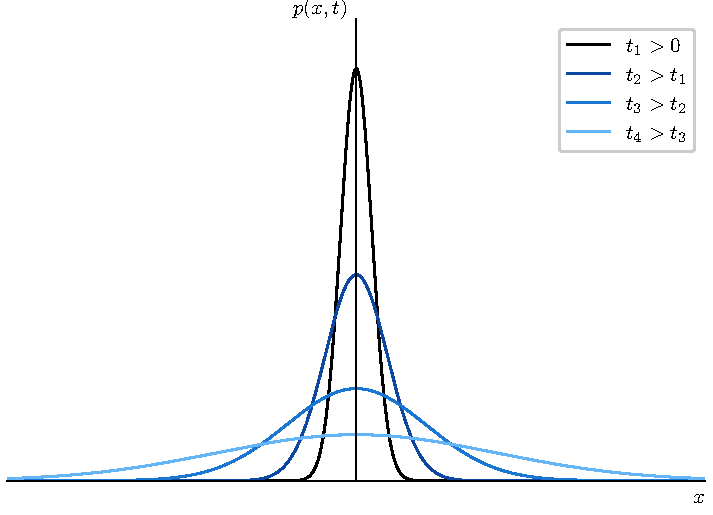
\includegraphics[width=0.8\textwidth]{images/gaussian_evolution.pdf}
    \caption{Evolution of the probability density $p(x,t)$ over time. Starting from a Dirac delta at $t=0$, the distribution spreads out as a Gaussian with variance $\sigma_t^2=2Dt$ increasing linearly in time.}
    \label{fig:gaussian_evolution}
\end{figure}


Another relevant quantity to characterize the displacement of the particle is the Mean Squared Displacement (MSD). It is defined as the average squared distance the particle has traveled from its starting point.
\begin{equation}
\text{MSD}(t) = \langle [x(t) - x(0)]^2 \rangle.
\end{equation}
Let's consider two cases:
\begin{itemize}
    \item If the particle starts at the origin, $x(0)=0$:
    \begin{equation}
    \text{MSD} = \langle [x(t)]^2 \rangle = \langle x^2(t) \rangle = 2Dt.
    \end{equation}
    The MSD is simply the variance.

    \item If the particle starts at a generic position $x(0)=x_0$:
    \begin{equation}\begin{split}
        \text{MSD} &= \langle [x(t) - x_0]^2 \rangle \\
        &= \langle x^2(t)\rangle + x_0^2 - 2x_0  \langle x(t)\rangle\\
        &= \langle x^2(t)\rangle + x_0^2 - 2x_0^2  \\
        & = x_0^2  + 2Dt - x_0^2 \\
        & = 2Dt.
    \end{split}\end{equation}
\end{itemize}
In both cases, the MSD grows linearly with time.

The typical distance traveled by the particle, the mean free path  $\lambda_x$, can be estimated as the root of the MSD.
\begin{equation}
\lambda_x = \sqrt{\text{MSD}} = \sqrt{2Dt}.
\end{equation}
This shows that the characteristic displacement of a diffusing particle grows not with time $t$, but with its square root. This sub-linear growth is a direct consequence of the random, back-and-forth nature of the motion.

\subsection{Einstein's second paper}

Let us now investigate the physical significance of the diffusion coefficient $D$.
We recall from the studies of R. Brown, that the motion of suspended (Brownian) particles becomes more intense as the temperature $T$ rises and as the viscosity $\eta$ of the liquid or the radius $R$ of the particles decrease.
Thus, we need to link these macroscopic parameters (the radius of the particle -- $\sim10^{-6}m$ -- is sufficiently large to neglect quantum effects and consider it a macroscopic object) to the diffusion coefficient.

Let us consider a statistical ensemble of $N$ identical Brownian particles of radius $R$, suspended in a three-dimensional tank liquid of temperature $T$ and viscosity $\eta$ in statistical equilibrium.
We consider three main forces acting on each particle in the vertical direction ($x$):
\begin{itemize}
	\item Gravitational pull:
	\begin{equation}
	F_G=-mg=-\frac{d}{dx}\bigl(V_G(x)\bigr), \qquad V_G(x)=mgx.
	\end{equation}
	\item Archimede's buoyancy:
	\begin{equation}
	F_A(x)=\rho(x)\, g\, Vol \ll F_G \qquad \text{(negligible)}.
	\end{equation}
	\item Stokes drag:
	\begin{equation}
	F_S=-6\pi\eta R v \qquad \text{(valid for low Reynolds' number)},
	\end{equation}
	where the factor $6\pi\eta R$ is also known as the \emph{mobility coefficient}.
	% CLAUDE NOTE: the annotation "coeff. di mobilità" appears in the handwritten notes
	% (PDF 1, page 7) and was previously missing from this section.
\end{itemize}
Restricting our attention to the stationary regime we can define a drift velocity of
\begin{equation}
v_d=\frac{F_G}{6\pi \eta R},
\end{equation}
and a superficial current of matter (number of particles that cross the unit of surface in the unit of time)
\begin{equation}
J_{drift}(x)=v_d\,\rho(x).
\end{equation}
Under the hypothesis of statistical equilibrium and classical physics, Boltzmann formula (see Appendix~\ref{app:ensembles}) entails that
\begin{equation}
\rho(E)=N\frac{e^{-\beta E}}{\mathcal{Z}}, \qquad \beta=(k_BT)^{-1}, \quad E=V(x)+\frac{mv^2}{2}.
\end{equation}
Hence, if we have that $\rho(0)=Ne^{-\beta m v^2/2}$ ($\iff V(0)=0$)
\begin{equation}
	\frac{\rho(x)}{\rho(0)}=e^{-\beta V(x)}.
\end{equation}
This is the case of the gravitational potential $V(x)=V_G(x)=mgx$, which recovers the so-called \textit{barometric distribution}
\begin{equation}
\rho(x)=\rho(0)e^{-\beta m g x}.
\end{equation}
% CLAUDE NOTE: written as in the handwritten notes (PDF 1, page 8), ρ(x) = e^{-βmgx};
% the earlier |F_G| intermediate step was removed at the author's request (2026-07-06).

Since the concentration of the Brownian particles increases with the depth of the liquid, each particle, while falling, experiences an increasing upward "force" generated by the consecutive scattering with other Brownian particles.
The analytic form of the current generated by this effect is nothing more than Fick's diffusion current
\begin{equation}
J_{diff}(x)=-D_{E.S.}\frac{d}{dx}\rho(x),
\end{equation}
for some $D_{E.S.}\in \mathbb{R}^+$ (this is Fick's first law; the second is the diffusion equation itself).
% CLAUDE NOTE: the parenthesis "(la II è quella eq. di diff.)" is in the notes (PDF 1,
% page 7) and was previously missing.
Considering the stationary regime, we demand $\rho(x)$ to be constant over time, \textit{i.e.}, with zero net flow $J_{diff}-J_{drift}=0$.
Identifying $V(x)=Fx$ for some constant force $F=F_G+F_S$,
\begin{equation}
-D\frac{d\rho(x)}{dx}-v_d\rho(x)=0,
\end{equation}
that is,
\begin{equation}
e^{-\beta Fx}\frac{F}{6\pi \eta R}=\rho(x)v_d=-D_{E.S.}\frac{d\rho(x)}{dx}=D_{E.S.}\beta F e^{-\beta F x},
\end{equation}
and simplifying the common exponential factor,
\begin{equation}
D_{E.S.} =\frac{k_BT}{6\pi\eta R},
\end{equation}
where "E.S." stands for Einstein-Smoluchowski.
As a consequence, the variance $\sigma_t^2=2D_{E.S.}t$ varies with the temperature $T$ and the viscosity $\eta$, exactly as in Brown's qualitative observations.
% CLAUDE NOTE: the sentence "dunque la varianza σ_t² varia con T,η" is in the notes
% (PDF 1, page 8) and was previously missing.
With this characterisation, we find all the properties of the chaotic motion described by R. Brown with the exception of self-similarity\footnote{See J. B. Perrin's work for an experimental verification of the Einstein-Smoluchowski formula\cite{Perrin1909}.
Measuring $D$ gives access to $k_B=R/N_A$, hence to an experimental measurement of Avogadro's number $N_A$, in great agreement with the chemical estimate; this earned Perrin the Nobel Prize in 1926.
% CLAUDE NOTE: the k_B = R/N_A remark is in the notes (PDF 1, page 8) and was
% previously missing from this footnote.
}.

Considering a statistical ensemble, we can identify $p(x,t)\leftrightarrow \rho(x,t)$.
% CLAUDE NOTE: the previous version wrote p(x,y), a typo for p(x,t).
Recalling the following formula for Einstein's first work
\begin{equation}\begin{split}
	& \partial_t\rho(x,t)=D\partial_x^2\rho(x,t)\implies\\
	& 0=\partial_t\rho(x,t)-\partial_x\{D\partial_x\rho(x,t)\}=\partial_t\rho(x,t)+\partial_x J(x,t),
\end{split}\end{equation}
recovering a continuity equation for $J(x,t)=-D\partial_x\rho(x,t)$.
In the stationary regime we set $\rho(x,t)\to \rho_S(x)$, entailing that $\partial_t\rho_S=0$ and consequently $\partial_xJ_S=0$.
In this setting, we find $J(x)=-D\partial_x\rho_S(x)$.
This observation fixes $D=D_{E.S.}$.


\section{The Langevin equation}

We now would like to extend Einstein's characterisation of the Brownian motion by describing the trajectory of the Brownian particles.
This, for obvious reasons, cannot be done in a deterministic way, but an attempt to delineate an average trajectory was made by Langevin: his reasoning goes as follows.
Langevin's equation (1908)\cite{Langevin1908} provides a \emph{microscopic} description of the motion, and it is historically the first \emph{stochastic differential equation} --- an object which, at the beginning, had no precise mathematical meaning, and was formalized only later.
% CLAUDE NOTE: the sentence above transcribes the notes' "eq. di Langevin (1908),
% descrizione microscopica → stoch. diff. eq., all'inizio non ha senso matematico,
% viene poi formalizzato" (PDF 1, page 9), previously missing. The formalization is
% the stochastic calculus of Chapter 4.

He considered a statistical ensemble of Brownian particles of mass $m$ and radius $R$ suspended in a 1-dimensional fluid of temperature $T$ and viscosity $\eta$ in statistical equilibrium.
Langevin admits a non-symmetric "jump" distribution, whose unbalance between the probability of a right and a left jump generates an overall drift velocity $v_d$.
The second principle of dynamics can be written as $ma=F=F^{(1)}+F^{(2)}$, with $F^{(1)}=F_S=-6\pi\eta Rv$ the deterministic Stokes force while $F^{(2)}=\xi(t)$ which models the stochastic particles scatterings as \textit{White Noise}.
We choose $\xi(t)$ such that for any time $t$ the ensemble average reads
\begin{equation}
	\langle \xi(t)\rangle_{Ensemble}=0, \;\mathrm{for}\,\,\mathrm{any}\; t\in \mathbb{R}.
\end{equation}
If we consider $\xi(t)\equiv 0$, we find a deterministic differential equation $m\frac{dv(t)}{dt}=-6\pi\eta R v(t)$, which has for a solution $v(t)=v(0)e^{-t/\tau}$, with $\tau=m/6\pi\eta R$.
Considering the full equation instead, it is problematic, because the trajectory it describes turns out not to be differentiable --- a difficulty ignored for the moment (we shall return to it in Chapter~3).
% CLAUDE NOTE: the remark "ma è problematico perché non è derivabile (ignorato per il
% momento)" is in the notes (PDF 1, page 10) and was previously missing.
We have
\begin{equation}\begin{split}
	&m\frac{d^2x}{dt^2}=-6\pi\eta R\frac{dx}{dt}+\xi(t)\\
	& mx\frac{d^2x}{dt^2}=-6\pi\eta Rx\frac{dx}{dt}+x\xi(t)
\end{split}\end{equation}
using the fact that $\frac{d(x^2)}{dt}=2x\frac{dx}{dt}$ and consequently $\frac{d(x^2)}{dt^2}=2(\frac{dx}{dt})^2+2x\frac{d^2x}{dt}$, we have
\begin{equation}\begin{split}
	&\bigg(\frac{m}{2}\bigg)\bigg(2x\frac{d^2x}{dt^2}\bigg)=\bigg(\frac{m}{2}\bigg)\bigg(\frac{d^2(x^2)}{dt^2}-2v^2\bigg),
\end{split}\end{equation}
then, substituting in the previous equation to express everything in function of $x^2$
\begin{equation}\begin{split}
	&\bigg(\frac{m}{2}\bigg)\frac{d^2(x^2)}{dt^2}-mv^2=-3\pi\eta R\frac{d(x^2)}{dt}+x\xi(t).
\end{split}\end{equation}
We observe that $x$ is a stochastic variable since it depends on $\xi(t)$.
In this spirit we evaluate the ensemble average of the differential equation, \textit{i.e.}
\begin{equation}\begin{split}
	&\bigg(\frac{m}{2}\bigg)\frac{d^2}{dt^2}\langle x^2 \rangle-\langle mv^2\rangle =-3\pi\eta R\frac{d}{dt}\langle x^2\rangle +\langle x\xi(t)\rangle.
\end{split}\end{equation}
We recall that under the hypothesis statistical equilibrium, it holds the Equipartition Theorem (Appendix~\ref{app:equipartition}), which entails that $\langle \frac{mv^2}{2}\rangle=\frac{k_BT}{2}$.
In addition, since $\xi(t)$ is independent from the particle's position (\textit{Markov process}), then we can factorise $\langle x\xi(t)\rangle =\langle x\rangle \langle \xi(t)\rangle=0$.
Collecting all of the above observations in one formula, gives
\begin{equation}\begin{split}
	\frac{m}{2}\frac{d^2}{dt^2}\langle x^2 \rangle +3\pi\eta R\frac{d}{dt}\langle x^2\rangle =k_BT.
\end{split}\end{equation}
We observe that, despite in the initial differential equation a stochastic term was added, in the final equation it does not appear: this is because we supposed $\langle \xi(t)\rangle =0$.
However, the trace of its existence lies in the fact that to erase the stochastic term, we had to consider an ensemble-average equation, giving up the "determinability" of our result.

If we set $f(t)=\frac{d}{dt}\langle x^2\rangle$, we have that
\begin{equation}\begin{split}
	&f'(t)+af(t)=b, \;a=6\pi\eta R/m, \;b=2k_BT/m\implies\\
	&f(t)=f_0(t)+f_p(t)=Ce^{-at}+b/a\implies\\
	&\frac{d}{dt}\langle x^2\rangle =Ce^{-\frac{6\pi\eta R t}{m}}+\frac{k_BT}{3\pi\eta R}=Ce^{-t/\tau}+\frac{k_BT}{3\pi\eta R},
\end{split}\end{equation}
with $\tau=m/6\pi\eta R\sim 10^{-8}s$.
After the transient state (\textit{i.e.} for $t>>\tau$) $e^{-t/\tau}\approx 0$, as a consequence, if we integrate the above equation on $[0,t]$ we have that
\begin{equation}\begin{split}
	\langle x^2(t)\rangle =\langle x^2(0)\rangle +\frac{k_BT}{3\pi\eta R}t=\langle x^2(0)\rangle +2t D_{E.S.}.
\end{split}\end{equation}
This result should make the reader "jump on their chair" since it explicitly confirms the equivalence of the macroscopic (statistical -- $p(x,t)$) derivation by Einstein-Smoluchowski with the microscopic (pseudo-deterministic -- $\langle x(t)\rangle$) derivation by Langevin.

The solutions of the Langevin equation constitute a \emph{family of time-dependent trajectories}.
Figure~\ref{fig:brownian-family} shows an ensemble of such trajectories: cutting the family at two successive times, the cross-sections of the cloud are Gaussians with larger and larger variance, exactly the $p(x,t)=\mathcal{N}(0,\,2Dt)$ of the macroscopic description.
% CLAUDE NOTE: "famiglia di traiettorie dipendenti dal tempo" + the pasted plot annotated
% "gaussiane con maggiore varianza" close the Langevin part of the notes (PDF 1, page 10);
% the figure below replaces the pasted plot.

% Figure generated by images/code_for_images/brownian_family.py
\begin{figure}[h!]
\centering
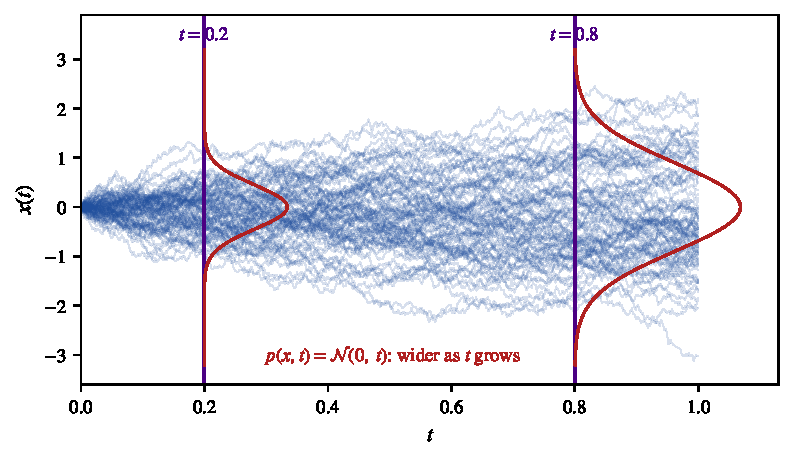
\includegraphics[width=0.85\textwidth]{images/brownian_family.pdf}
\caption{A family of Brownian trajectories, cut at two successive times $t_1=0.2$ and $t_2=0.8$ (vertical lines). The cross-section profiles (red) are Gaussians with variance growing linearly in time --- the microscopic trajectories reconstruct the spreading density of Figure~\ref{fig:gaussian_evolution}. Generated by \texttt{images/code\_for\_images/brownian\_family.py}.}
\label{fig:brownian-family}
\end{figure}


\section{The random walk of Bachelier}

The jump description of Brownian motion admits a discrete formulation of independent interest: the \emph{random walk}.
It was introduced for the first time by Bachelier in his PhD thesis \emph{Th\'eorie de la sp\'eculation} (1900)\cite{Bachelier1900} --- five years \emph{before} Einstein's papers, and with prices, not pollen grains, in mind.

The model rests on four hypotheses.
\begin{enumerate}[label=\roman*)]
    \item The particle can occupy equispaced cells (of width $\Delta x$) on a one-dimensional lattice extending over $(-\infty,+\infty)$.
    \item The initial position is zero at $t=0$.
    \item Calling $P$ the probability of jumping to the right and $q$ the one of jumping to the left, one has $P+q=1$, and the jumps occur regularly, once every interval $\Delta t$.
    (For Einstein, $P=q$.)
    \item The jumps are independent (Markov).
\end{enumerate}
The position is labelled by $m\in\mathbb{Z}$ and $N\in\mathbb{N}$ is the number of jumps performed, so that $N\Delta t$ is the elapsed time.

\begin{center}
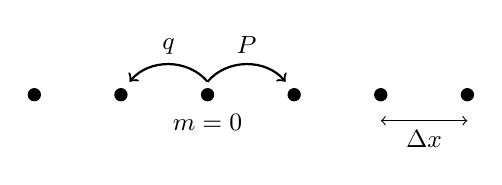
\begin{tikzpicture}[scale=1.1]
  \foreach \x in {-2,-1,0,1,2,3}{ \filldraw[black] (\x,0) circle (2pt); }
  \draw[->, thick] (0,0.15) to[bend left=50] node[above]{\small $P$} (0.9,0.15);
  \draw[->, thick] (0,0.15) to[bend right=50] node[above]{\small $q$} (-0.9,0.15);
  \node[below] at (0,-0.12) {\small $m=0$};
  \draw[<->] (2,-0.3) -- (3,-0.3) node[midway, below]{\small $\Delta x$};
\end{tikzpicture}
\end{center}

The question is: what is the probability distribution $P_N(m)$ of being at position $m$ after $N$ jumps?
If $P=\tfrac{1}{2}=q$ the model is the \emph{symmetric} random walk; for $P\ne\tfrac{1}{2}$ and $q=1-P$ the individual jumps are Bernoulli variables, and their sum follows a \emph{binomial distribution}.
The counting is elementary: if the walker performs $m+\ell$ jumps to the right, it must perform $\ell$ jumps to the left, hence $N=m+2\ell$ jumps in total; solving,
\begin{equation}
\ell=\frac{N-m}{2} \ \text{ jumps to the left},
\qquad
m+\frac{N-m}{2}=\frac{N+m}{2} \ \text{ jumps to the right},
\end{equation}
and the binomial distribution is then
\begin{equation}
P_N(m) = \binom{N}{\frac{N+m}{2}}\, P^{\frac{1}{2}(N+m)}\, q^{\frac{1}{2}(N-m)}.
\end{equation}
Normalizing the price to zero at $t=0$, this can be taken as a model for the evolution of prices --- Bachelier's original purpose.

To compute the moments it is convenient to introduce the number of right jumps
\begin{equation}
r:=\frac{N+m}{2},
\qquad
P_N(r)=\binom{N}{r}P^r q^{N-r} = \mathcal{B}(r;P,N),
\end{equation}
for which the standard binomial results follow.
The normalization is immediate from the binomial theorem,
\begin{equation}
\sum_{r=0}^{\infty}\binom{N}{r}P^r q^{N-r} = (P+q)^N = 1,
\end{equation}
the mean is
\begin{equation}
\mathbb{E}[r]=\sum_{r=0}^{\infty} r\,P_N(r) = NP,
\end{equation}
and, from $\mathbb{E}[r^2]=NP+N(N-1)P^2$, the variance is
\begin{equation}
\mathrm{Var}[r]= NP+N(N-1)P^2-N^2P^2 = NP(1-P).
\end{equation}
Translating back to the position through $m=2r-N$,
\begin{equation}
\langle m\rangle = 2\langle r\rangle - N = 2NP-N = 2N\Bigl(P-\frac{1}{2}\Bigr),
\qquad
\mathrm{Var}[m] = 4NP(1-P),
\end{equation}
where we used $\langle m^2\rangle = 4NP(1-P)+4N^2(P-\tfrac{1}{2})^2$.

Both the mean and the variance depend linearly on $N$; but $N=t/\Delta t$, so they are \emph{linear in time} --- recall Einstein's $\sigma_E^2=2Dt$, whose mean vanished because $P=q=\tfrac{1}{2}$.
% CLAUDE NOTE: the notes write "(si ricordi σ_E² = 2Dt, σ_E = 0 perché P=q=½)" (PDF 1,
% page 12); as written, σ_E=0 would contradict σ_E²=2Dt. The intended statement is that
% the MEAN ⟨m⟩ vanishes in the symmetric (Einstein) case, as rendered above.
Note, moreover, that the distribution is a binomial, \emph{not} a Gaussian.

The role of the asymmetry is best seen in three regimes, sketched in Figure~\ref{fig:rw-regimes}.
In the \emph{maximally asymmetric} model ($P=1$, $q=0$, or $P=0$, $q=1$) one has $\mathrm{Var}[m]=0$ and $\mathbb{E}[m]=\pm N$: the walk is purely deterministic.
With $P=\tfrac{3}{4}$, $q=\tfrac{1}{4}$ one finds $\langle m\rangle = N/2$ and $\mathrm{Var}[m]=\tfrac{3}{4}N$: the variable fluctuates around a rising trend.
Finally, with $P=q=\tfrac{1}{2}$, $\langle m\rangle = 0$ and $\mathrm{Var}[m]=N$: pure fluctuation, with the $\sqrt{N}$ fan-out of diffusion.

\begin{figure}[h!]
\centering
\begin{tikzpicture}[scale=0.9]
  % panel 1: deterministic
  \begin{scope}
    \draw[->] (0,0) -- (2.6,0) node[right]{\small $N$};
    \draw[->] (0,-1.3) -- (0,1.5) node[above]{\small $m$};
    \draw[dotted, thick, blue!60!black] (0,0) -- (2.4,1.2) node[right]{\small $\langle m\rangle$};
    \draw[dotted, thick, olive] (0,0) -- (2.4,-1.2) node[right]{\small $\langle m\rangle$};
    \node[below] at (1.3,-1.5) {\small $P=1$ or $q=1$};
  \end{scope}
  % panel 2: asymmetric fluctuating
  \begin{scope}[xshift=5.2cm]
    \draw[->] (0,0) -- (2.6,0) node[right]{\small $N$};
    \draw[->] (0,-1.3) -- (0,1.5) node[above]{\small $m$};
    \draw[dashed] (0,0) -- (2.4,1.0);
    \draw[thick] (0,0) -- (0.3,0.3) -- (0.5,0.1) -- (0.8,0.55) -- (1.0,0.35)
       -- (1.3,0.75) -- (1.5,0.5) -- (1.8,0.95) -- (2.0,0.7) -- (2.3,1.1);
    \node[below] at (1.3,-1.5) {\small $P=\tfrac34,\ q=\tfrac14$};
  \end{scope}
  % panel 3: symmetric
  \begin{scope}[xshift=10.4cm]
    \draw[->] (0,0) -- (2.6,0) node[right]{\small $N$};
    \draw[->] (0,-1.3) -- (0,1.5) node[above]{\small $m$};
    \draw[dotted] (0,0) parabola (2.4,1.1);
    \draw[dotted] (0,0) parabola (2.4,-1.1);
    \draw[thick] (0,0) -- (0.25,0.25) -- (0.45,-0.1) -- (0.7,0.3) -- (0.95,-0.2)
       -- (1.2,-0.55) -- (1.45,-0.25) -- (1.7,-0.7) -- (1.95,-0.35) -- (2.3,0.4);
    \node[below] at (1.3,-1.5) {\small $P=q=\tfrac12$};
  \end{scope}
\end{tikzpicture}
\caption{The three regimes of the random walk: purely deterministic ($P=1$ or $q=1$, zero variance), asymmetric (fluctuations around a linear trend), and symmetric (pure fluctuation inside the $\pm\sqrt{N}$ envelope).}
\label{fig:rw-regimes}
\end{figure}

But this --- Samuelson observed --- cannot be an acceptable model for the fluctuation of prices, because the fluctuations would decrease, which is not what happens.
% CLAUDE NOTE: the notes read "Ma questo (Samuelson) non può essere un modello accettabile
% per la fluttuazione dei prezzi perché le fluttuazioni calerebbero, cosa che non accade"
% (PDF 1, page 12). The explanatory paragraph and the numerical example below were added
% at the author's request (2026-07-06).
The objection deserves to be spelled out, because it is precisely the observation that will lead to the geometric model of Chapter~4.
In an asymmetric random walk the mean position grows linearly, $\langle m\rangle \propto N$, while the spread grows only as a square root, $\mathrm{s.d.}[m] = \sqrt{4NPq} \propto \sqrt{N}$; the fluctuations \emph{relative to the price level} therefore decay,
\begin{equation}
\frac{\mathrm{s.d.}[m]}{\langle m\rangle} \propto \frac{\sqrt{N}}{N} = \frac{1}{\sqrt{N}} \;\xrightarrow{\ N\to\infty\ }\; 0,
\end{equation}
and an asset following this model would become, in proportion to its own value, ever quieter as it grows.
A concrete example makes the failure vivid.
Take a stock worth 100\,\euro{} today, fluctuating by about 1\,\euro{} per day (one percent), and suppose that over the years its price drifts up tenfold, to 1000\,\euro.
The arithmetic model predicts that its daily fluctuations are \emph{still} of the order of 1\,\euro{} --- now a mere $0.1\%$ of the price --- whereas a real thousand-euro stock keeps fluctuating by percentage points, that is, by tens of euros per day.
What is statistically stationary in real markets is the \emph{relative} return, not the absolute increment: the fluctuations must be proportional to the price itself, which is exactly the multiplicative structure of the geometric Brownian motion of Chapter~4.

\subsection{The continuum limit}

The Gaussian is recovered from the binomial in the \emph{continuum limit}.
Define the physical variables
\begin{equation}
x:=m\Delta x, \qquad t:=N\Delta t,
\end{equation}
so that the mean position becomes
\begin{equation}
\langle x\rangle = \langle m\rangle\,\Delta x = (2P-1)N\Delta x = (2P-1)\frac{t}{\Delta t}\Delta x,
\end{equation}
and, introducing the velocity
\begin{equation}
v:=\lim_{\substack{\Delta x\to0\\ \Delta t\to0}} (2P-1)\frac{\Delta x}{\Delta t}
\qquad \text{(the limit does not exist by itself: it is heuristic)},
\end{equation}
one finds $\langle x\rangle = v\,t$: a \emph{drift} term.
For the variance,
\begin{equation}
\mathrm{Var}[x] = \bigl\{\langle m^2\rangle - \langle m\rangle^2\bigr\}(\Delta x)^2 = 4Pq\,(\Delta x)^2\frac{t}{\Delta t},
\end{equation}
and defining the diffusion coefficient
\begin{equation}
D := \lim_{\substack{\Delta x\to0\\ \Delta t\to0}} 2Pq\,\frac{(\Delta x)^2}{\Delta t},
\qquad\text{it follows that}\qquad
\mathrm{Var}[x]=2Dt.
\end{equation}

The Gaussian solution is contained in Bachelier's model.
Indeed, for $P$ fixed and $N\to\infty$,
\begin{equation}
P_N(m)=\mathcal{B}(m;P,N) \;\longrightarrow\; P_G(m),
\qquad
P_G(m) = \frac{1}{\sqrt{2\pi\,4NPq}}\,\exp\Bigl\{-\frac{(m-\langle m\rangle)^2}{2\,(4NPq)}\Bigr\},
\end{equation}
a correctly normalized Gaussian: this is a particular case of the central limit theorem, known as the \emph{De Moivre--Laplace theorem}.
Passing to the physical variables, $m\to x=m\Delta x$ and $N\to t=N\Delta t$, some algebra and the continuum limit give
\begin{equation}
P_N(m,N) \;\longrightarrow\; P_N(m\Delta x, N\Delta t)\,\Delta x
\;\xrightarrow[\Delta t\to0]{\Delta x\to0}\;
\frac{1}{\sqrt{4\pi Dt}}\,\exp\Bigl\{-\frac{(x-vt)^2}{4Dt}\Bigr\}\,dx = P_G(x,t)\,dx,
\end{equation}
a Gaussian with $\langle x\rangle = vt$ and $\mathrm{Var}[x]=2Dt$: Einstein's solution, with a drift.

\subsection{From the master equation to the Fokker--Planck equation}

But where does this Gaussian come from?
In the discrete case, the probability of being at $x$ at time $t+\Delta t$ obeys the \emph{master equation}
\begin{equation}
P(x,t+\Delta t) = P\,P(x-\Delta x,t) + q\,P(x+\Delta x,t),
\end{equation}
since the walker must arrive either from the left (with probability $P$) or from the right (with probability $q$).
Expanding the left side in time,
\begin{equation}
P(x,t+\Delta t) = P(x,t) + \Delta t\,\frac{\partial P}{\partial t},
\end{equation}
and each term on the right in space,
\begin{equation}\begin{split}
P\,P(x-\Delta x,t) + q\,P(x+\Delta x,t)
&= P\Bigl[P(x,t) - \Delta x\frac{\partial P}{\partial x} + \frac{\Delta x^2}{2}\frac{\partial^2 P}{\partial x^2}\Bigr]\\
&\quad + q\Bigl[P(x,t) + \Delta x\frac{\partial P}{\partial x} + \frac{\Delta x^2}{2}\frac{\partial^2 P}{\partial x^2}\Bigr],
\end{split}\end{equation}
which reassembles into
\begin{equation}
\underbrace{(P+q)}_{=1} P(x,t) + \underbrace{(-P+q)}_{1-2P}\,\Delta x\,\frac{\partial P}{\partial x} + \underbrace{(P+q)}_{=1}\,\frac{\Delta x^2}{2}\,\frac{\partial^2 P}{\partial x^2}.
\end{equation}
Therefore, dividing by $\Delta t$ (the terms $P(x,t)/\Delta t$ cancel between the two sides),
\begin{equation}
\frac{\partial P}{\partial t} = (1-2P)\frac{\Delta x}{\Delta t}\frac{\partial P}{\partial x} + \frac{1}{2}\frac{\Delta x^2}{\Delta t}\frac{\partial^2 P}{\partial x^2},
\end{equation}
and with the definitions of $v$ and $D$ given above (with $P=q=\tfrac12$), in the continuum\footnote{A small bookkeeping subtlety: the expansion produces the diffusion coefficient $\tfrac12\Delta x^2/\Delta t$, while the variance-based definition given earlier is $D = 2Pq\,\Delta x^2/\Delta t$; the two coincide exactly at $P=q=\tfrac12$ ($4Pq=1$), which is why the derivation specifies this case.
In the joint limit $\Delta x,\Delta t\to0$ with $v$ and $D$ finite, $P\to\tfrac12$ automatically, so no inconsistency survives in the continuum.}
% CLAUDE NOTE: the bookkeeping remark was promoted from a source comment to the footnote
% above at the author's request (2026-07-06).
\begin{equation}
\frac{\partial}{\partial t}P(x,t) = \underbrace{D\frac{\partial^2}{\partial x^2}P(x,t)}_{\text{pure diffusion}} - \underbrace{v\frac{\partial}{\partial x}P(x,t)}_{\text{drift}},
\end{equation}
without the drift term when $\langle x\rangle=0$.
This is the \emph{Fokker--Planck equation} --- here obtained for the simplest of all processes, and derived in full generality in Chapter~3.


\section{The central limit theorem}

The Gaussian appeared twice in this chapter --- as the solution of the diffusion equation and as the limit of the binomial --- and this is no coincidence: behind both stands the \emph{central limit theorem} (CLT), which we now state, prove, and (importantly for what comes later in this book) criticize.

\medskip
\noindent\textbf{Theorem (CLT).}
\emph{Let $\{X_i\}_i$ be random variables and $S_N:=\sum_{i=1}^{N}X_i$ their sum; then, for $N\to\infty$, $S_N$ tends to a Gaussian, provided that (a) the $X_i$ are i.i.d.\ (independent and identically distributed), and (b) the mean $\langle X_i\rangle$ and the variance $\mathrm{Var}[X_i]$ exist finite for every $i$.}
\medskip

The two hypotheses look innocent; the critique of L\'evy and Mandelbrot, to which we return at the end of the section, is aimed precisely at them.

\subsection{Characteristic functions}

The proof (due to Lindeberg and L\'evy) rests on the \emph{characteristic function}: given a density $P(x)$ on $\mathbb{R}$,
\begin{equation}
\varphi(k) := \int_{\mathbb{R}} dx\, e^{ikx}\,P(x) = \mathcal{F}[P] = \mathbb{E}\bigl[e^{ikx}\bigr],
\qquad
P(x) = \frac{1}{2\pi}\int_{\mathbb{R}} dk\, e^{-ikx}\,\varphi(k),
\end{equation}
i.e.\ the Fourier transform of the density.
Two properties make it the perfect tool.

\paragraph{a) Convolution theorem.}
Since $\mathcal{F}[f*g]=\mathcal{F}[f]\cdot\mathcal{F}[g]$, sums of independent variables become products of characteristic functions.
Explicitly: for $X_1$ and $X_2$ i.i.d., the sum $S_2:=X_1+X_2$ is again random, and its density is obtained by extracting the two variables, $P(x_1,x_2)=P(x_1)P(x_2)=P(S_2-x_1)P(x_1)$, and summing over all the possible ways of realizing $S_2$:
\begin{equation}
P_2(S_2)=\int_{\mathbb{R}} P(S_2-x_1)\,P(x_1)\,dx_1,
\end{equation}
the convolution of two identical densities.
Transforming,
\begin{equation}
\mathcal{F}[P_2]=\mathcal{F}[P*P]=\varphi_2(k)=\mathcal{F}[P]\,\mathcal{F}[P]=\varphi^2(k),
\end{equation}
and iterating,
\begin{equation}
\mathcal{F}[P_N]=\varphi_N(k)=\varphi^N(k).
\end{equation}

\paragraph{b) Moment expansion.}
Expanding $e^{ikx}=\sum_{m=0}^{\infty}\frac{(ik)^m}{m!}x^m$ inside the transform,
\begin{equation}
\varphi(k)=\int_{\mathbb{R}} dx\, e^{ikx}P(x) = \sum_{m=0}^{\infty}\frac{(ik)^m}{m!}\int_{\mathbb{R}} dx\, x^m P(x) = \sum_{m=0}^{\infty}\frac{(ik)^m}{m!}\langle x^m\rangle,
\end{equation}
\emph{only if the moments exist} (i.e.\ the integrals converge) --- but it happens that infinitely many do not~(!), and this is where the critique will strike.
Conversely, the moments are read off the derivatives at the origin:
\begin{equation}
\frac{d^\ell}{dk^\ell}\varphi(k)\Big|_{k=0} = i^\ell\int_{\mathbb{R}} dx\, x^\ell\,P(x) = i^\ell\langle x^\ell\rangle
\quad\Longrightarrow\quad
\langle x^\ell\rangle = (-i)^\ell\,\frac{d^\ell}{dk^\ell}\varphi(k)\Big|_{k=0},
\qquad \forall\,\ell,
\end{equation}
% CLAUDE NOTE: the notes write "⟨x^ℓ⟩ = −i^ℓ d^ℓ/dx^ℓ φ(k)|_{k=0}" (PDF 1, page 16):
% the derivative is with respect to k (not x), and the prefactor is (−i)^ℓ; both slips
% of fast handwriting, rendered correctly above.
so that from $\varphi(k)$ one reconstructs the whole distribution.

\subsection{Proof of the theorem}

We standardize first.
Let $\mu:=\langle X_i\rangle$ and $\sigma^2:=\mathrm{Var}[X_i]$ (equal for all $i$ because the variables are identically distributed, but the argument generalizes), and define
\begin{equation}
X_i \;\longrightarrow\; \xi_i := \frac{X_i-\mu}{\sigma},
\qquad
\langle\xi_i\rangle = 0, \quad \mathrm{Var}[\xi_i]=1,
\end{equation}
rescaling then each variable by $\sqrt{N}$, $\xi_i\mapsto \xi_i/\sqrt{N}$.
The standardized sum
\begin{equation}
S_N := \frac{1}{\sqrt{N}}\sum_{i=1}^{N}\xi_i,
\qquad
\langle S_N\rangle = \frac{1}{\sqrt{N}}\sum_i \langle\xi_i\rangle = 0,
\quad
\mathrm{Var}[S_N] = \langle S_N^2\rangle = \frac{1}{N}\sum_{i=1}^{N}\langle\xi_i^2\rangle = 1,
\end{equation}
remains itself standardized.
We must show that $P(S_N)=P_G(S_N)=\mathcal{N}(0,1)$, and we do so by showing that the two have the same characteristic function.

Each rescaled variable contributes $\mathbb{E}\bigl[e^{ik\xi_i/\sqrt{N}}\bigr]=\varphi\bigl(\tfrac{k}{\sqrt{N}}\bigr)$ for every $\xi_i$, so by the convolution theorem
\begin{equation}
\varphi_N(k) = \Bigl[\varphi\Bigl(\frac{k}{\sqrt{N}}\Bigr)\Bigr]^{N}.
\end{equation}
Expanding in moments,
\begin{equation}
\varphi\Bigl(\frac{k}{\sqrt{N}}\Bigr) \approx 1 + \frac{ik}{\sqrt{N}}\underbrace{\langle\xi_i\rangle}_{=0} - \frac{k^2}{2N}\underbrace{\mathrm{Var}[\xi_i]}_{=1} - \frac{i}{3!}\frac{k^3}{N^{3/2}}\langle\xi_i^3\rangle + \frac{1}{4!}\frac{k^4}{N^2}\langle\xi_i^4\rangle + \dots,
% CLAUDE NOTE: the notes (PDF 1, page 16) write the third and fourth terms with flipped
% signs (+i/3!... and −1/4!...); corrected here at the author's request (2026-07-06),
% since (ik)³ = −ik³ and (ik)⁴ = +k⁴. The slip was inconsequential, as these terms are
% suppressed for N→∞ and dropped in the next step.
\end{equation}
where $\langle\xi_i^3\rangle$ is the \emph{skewness}, the parameter of asymmetry (zero if the distribution is symmetric), and $\langle\xi_i^4\rangle$ is the \emph{kurtosis}, the parameter of the behaviour of the tails (heavy tails).
Almost all the known distributions have their higher moments defined, and for large $N$ these are negligible with respect to the first two; therefore
\begin{equation}
\varphi_N(k) \approx \Bigl(1-\frac{k^2}{2N}\Bigr)^{N},
\qquad
\lim_{N\to\infty}\varphi_N(k) = \lim_{N\to\infty}\Bigl(1-\frac{k^2}{2N}\Bigr)^{N} = e^{-k^2/2},
\end{equation}
using $(1+\tfrac{a}{x})^x\xrightarrow{x\to\infty}e^a$.
Inverting the transform, by completing the square exactly as in the solution of the diffusion equation,
\begin{equation}\begin{split}
P(S_N) &= \frac{1}{2\pi}\int_{\mathbb{R}} dk\, e^{-k^2/2}\,e^{-ikS_N}\\
&= \frac{1}{2\pi}\int_{\mathbb{R}} dk\, e^{-\frac{1}{2}(k+iS_N)^2}\,e^{-S_N^2/2}
= \frac{1}{\sqrt{2\pi}}\,e^{-S_N^2/2}:
\end{split}\end{equation}
a Gaussian with mean $0$ and variance $1$. $\blacksquare$

\subsection{Critical remarks}

The theorem is powerful, but each of its hypotheses deserves interrogation --- and the answers open the door to the econophysics of Chapter~7.
\begin{itemize}
    \item \emph{Does it hold if the variables are not independent?} No.
    \item \emph{If they are not identically distributed?} Yes --- but no single variable must dominate the others.
    \item \emph{Is the asymptotic limit necessary?} No (the Berry--Esseen theorem controls the finite-$N$ error), but the summands must be \emph{stable}: invariant in form under addition and convolution.
    \item \emph{Can it hold if the mean and/or the variance do not exist?} No.
    Do similar PDFs exist? Yes: the \emph{L\'evy-stable distributions} --- which turn out to be better at describing real data.
    And does a form of the theorem exist for variables drawn from L\'evy-stable laws? Yes: the \emph{generalized CLT}, whose limit is not a Gaussian.
    \item \emph{If mean, variance and skewness exist, but the kurtosis does not, does the CLT hold?}
    There exist distributions of this kind: e.g.\ the Student-$t$, $P_S(x,\nu)$, with $\nu$ degrees of freedom, for which $\nu\to\infty$ gives $P_S\to P_G(0,1)$; or the Tsallis distribution, $P_t(x,q)\xrightarrow{q\to1}\mathcal{N}(0,1)$; here $q,\nu$ are shape parameters.
    Such distributions are \emph{leptokurtic}: sharper at the centre and heavier in the tails than the Gaussian (Figure~\ref{fig:leptokurtic}; the case $\nu=3$ will star in Chapter~7).
    The sum of many $P_S$ variables does reproduce a Gaussian \emph{at the centre} --- which makes sense, since mean and variance refer to the central part --- but the convergence is very slow (sums of order $10^2$).
\end{itemize}

\begin{figure}[h!]
\centering
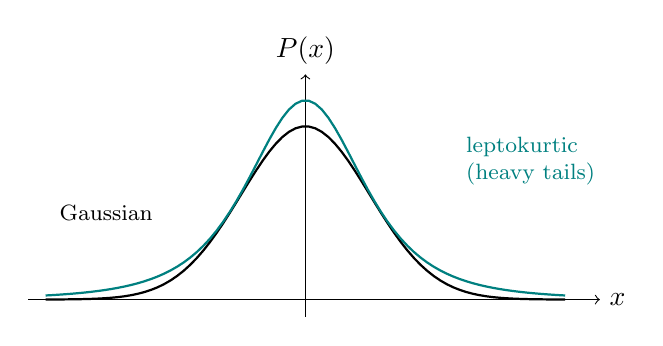
\begin{tikzpicture}[scale=1.1]
    \draw[->] (-3.2,0) -- (3.4,0) node[right]{$x$};
    \draw[->] (0,-0.2) -- (0,2.6) node[above]{$P(x)$};
    \draw[thick, domain=-3:3, samples=80] plot (\x, {2.0*exp(-\x*\x/1.1)});
    \draw[thick, teal, domain=-3:3, samples=80] plot (\x, {2.3/((1+\x*\x/1.5)^2)});
    \node[teal, font=\footnotesize, align=left] at (2.6,1.6) {leptokurtic\\ (heavy tails)};
    \node[font=\footnotesize] at (-2.3,1.0) {Gaussian};
\end{tikzpicture}
\caption{A leptokurtic distribution (teal) against a Gaussian of the same scale: sharper peak at the centre, heavier tails far out. Sums of such variables re-Gaussianize only in the central region, and very slowly.}
\label{fig:leptokurtic}
\end{figure}

The most famous L\'evy-stable law is the \emph{Cauchy} distribution,
\begin{equation}
P_c(x)=\frac{\gamma}{\pi}\,\frac{1}{x^2+\gamma^2},
\qquad \gamma \text{ of scale},
\end{equation}
for which the pathology can be checked by hand: with $\gamma=1$,
\begin{equation}\begin{split}
\langle x^2\rangle &= \frac{1}{\pi}\int_{\mathbb{R}} x^2\,\frac{1}{x^2+1}\,dx\\
&= \frac{2}{\pi}\biggl\{\int_0^{\infty}\!dx\,\frac{x^2+1}{x^2+1} - \int_0^{\infty}\!dx\,\frac{1}{x^2+1}\biggr\}\\
&= \frac{2}{\pi}\Bigl[x-\arctan x\Bigr]_0^{+\infty} = +\infty,
\end{split}\end{equation}
and $\langle x\rangle = \infty$ --- more precisely, the integral defining the mean is not absolutely convergent (its principal value is zero), so the mean is in fact \emph{undefined} rather than infinite.
% CLAUDE NOTE: the notes write "⟨x⟩ = ∞" (PDF 1, page 17); the clarification about
% absolute convergence was promoted from this comment into the text at the author's
% request (2026-07-06). The second moment is genuinely +∞.
More generally, a L\'evy-stable density $P_\alpha(x)$ behaves asymptotically as
\begin{equation}
P_\alpha(x) \;\xrightarrow{|x|\to\infty}\; \frac{1}{|x|^{1+\alpha}},
\qquad 0<\alpha\le2,
\end{equation}
interpolating between the Gaussian ($\alpha=2$) and pure power laws: for $0<\alpha<1$ neither the mean nor the variance exist; for $1<\alpha<2$ the variance does not exist.
And summing Cauchy variables? Still a Cauchy: the L\'evy-stable laws \emph{replicate themselves} under addition --- they are the fixed points that the generalized CLT converges to, as the Gaussian is for the classical one.
All of this is taken up quantitatively in Chapter~7, where these distributions meet financial data.

Mandelbrot's verdict on the classical hypotheses may serve as the epigraph for that chapter: \emph{``physicists think the whole world is Gaussian''}.
